\documentclass[oneside]{book}

% Cover Variables
	\newcommand{\ctitle}{Transmission par Fibre Optique}
	\newcommand{\cautor}{Jules Fellouse - Lucas Lescure}

% Header Variables
	\newcommand{\headRE}{\textbf{ \leftmark}}
	\newcommand{\footRE}{\text{\rightmark}}
	\newcommand{\footLE}{\textbf{Page \thepage}}

% TOC Variables
	\newcommand{\toctitle}{Table des contenus}
	\newcommand{\tocchapter}{Partie}
	\newcommand{\toccount}{2}

% Chapter Variables
	\newcommand{\chvar}{Partie -}

\input{\string~/Projects/common/.style.tex}

\input{\string~/Projects/common/.math.tex}

\input{\string~/Projects/common/.header.tex}
	
\input{\string~/Projects/common/.toc.tex}

% figure support
\usepackage{import}
\usepackage{xifthen}
\pdfminorversion=7
\usepackage{pdfpages}
\usepackage{transparent}
\newcommand{\incfig}[1]{%
	\def\svgwidth{\columnwidth}
	\import{./figures/}{#1.pdf_tex}
}

\pdfsuppresswarningpagegroup=1

\patchcmd{\thebibliography}{\chapter}{\subsection}{}{}
\renewcommand{\bibname}{Bibliographie}

\begin{document}
	% Spacing 
	\input{\string~/Projects/common/.begin.tex}

	% Cover
	\input{\string~/Projects/common/.cover.tex}
	
	\vfill
	\subsection*{Abstrait}
	La fibre optique est beaucoup utilisée dans la télécommunication pour transmettre des informations sur de longues distances. On cherche donc à savoir comment c'est réalisable en s'intéressant au fonctionnement des composants essentiels qui interviennent dans cette transmission. En particulier sur le multiplexage, la modulation et la fibre optique. On utilisera les notions acquises dans le but de recréer cette transmission et comprendre comment la lumière peut-être utilisée comme porteuse d'une information.  

	\newpage

	\thispagestyle{nohead}

	\section{Introduction}
	Suite à l'invention du laser en 1960 par le physicien Théodore Maiman et l'amélioration des fibres optiques, la transmission par fibre optique a révolutionné la monde de la télécommunication. Aujourd'hui c'est le moyen le plus utilisé en raison de sa faible atténuation par rapport au fil de cuivre. Sur 100 mètres la fibre optique subit une atténuation de 3\% tandis que sur la même distance un fil de cuivre porte une atténuation de 90\%\cite{attenuation}. De plus, une transmission par fil de cuivre est contrainte à subir des perturbations en raison des interférences électromagnétiques, les différences de température qui varies la résistance du fil. En haute fréquences il est presque impossible d'envoyer des données sur des longues distances par le biais de son atténuation, il lui faut de nombreux répéteurs. En contraste, la fibre optique est capable de transmettre un signal sur des kilomètres avec un débit de l'ordre des $\ds{1000\ Go/s}$ par rapport au cuivre qui ne peut pas transmettre plus loins que 100 mètres avec un débit de $\ds{100\ Mo/s}$(source?).


	\begin{figure}[ht!]
		\centering
		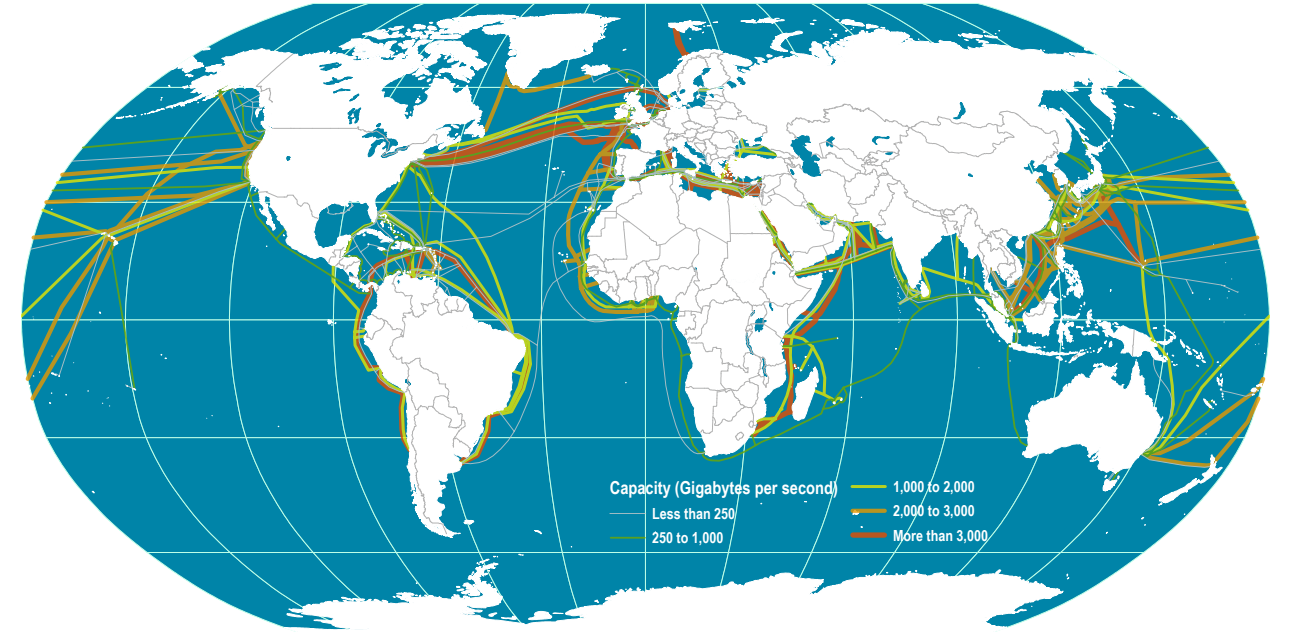
\includegraphics[width=0.8\textwidth]{./object/submarine.png}
		\caption{Carte des câbles sous-marin de télécommunication}
		\label{fig:submarine}
	\end{figure}

	Ces chiffres sont atteignables grâce aux propriétés de la fibre optique et à des techniques de multiplexage qui permettent d'envoyer plusieurs signaux sur un même fil utilisant l'entièreté de la bande passante disponible.
	Cependant il reste à comprendre comment la lumière est utilisée pour transmettre des donnés dans une transmission par fibre optique.

	Pour ceci nous nous intéresserons premièrement à la façon d'envoyer un signal optique en utilisant un modulateur. Ensuite nous  chercherons un moyen de transmettre plusieurs signaux sur une même fibre en étudiant les different types de multiplexeurs ainsi que leur fonctionnement. Nous verrons ensuite comme cette donnée se propage à l'intérieur de certaines fibres pour en choisir une adaptée à une transmission de longue distance. Grâce à tout cela nous pourrons alors étudier en detail la configuration des réseaux PON et établir notre propre modèle de transmission. 

	\chapter{Modulation}
		
		\section{Modulation Directe}

		\section{Modulation Externe}



	\chapter{MULTIPLEXAGE}

	\vspace{-40pt}
	
		Comme nous avons vu dans la \underline{Propagation} (add ref), la fibre optique possède un bande passante dans laquelle on retrouve les longueurs d'onde les moins atténués et qui seront donc utilisés pour la propagation d'information. C'est cette bande passante que l'on va pouvoir exploiter pour faire passer des téraoctets de donnés grâce aux multiplexage assurant que toute la bande passante soit utilisé . 

		Après la modulation de plusieurs signaux grâce à un modulateur externe on cherche à combiner ces différentes longueurs d'onde sur une même fibre. Soit disant il s'agit de prendre un démultiplexeur et inverser son sens. Dans ce raisonnement on traitera les démultiplexeur, en appliquant le sens inverse pour les multiplexeur.

		Il existe principalement 3 types de multiplexage, le multiplexage en longueur d'onde, en polarité, et temporel. En anglais, wave division multiplexing (WDM), polarisation division multiplexing (PDM) et time division multiplexing (TDM). \\
		Chaque type de multiplexage sera traité mais nous nous intéresserons plus au WDM car c'est celui le plus utilisé et le plus important pour traiter des donnés optiques. 



		\section{Multiplexage en longueur d'onde (WDM)}


			\begin{figure}[ht!]
				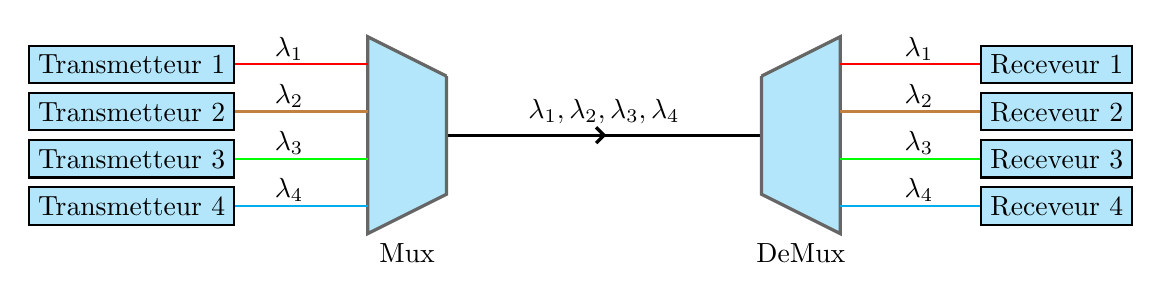
\begin{tikzpicture}
					\draw[very thick] (-2,0) -- (2,0); \draw[very thick] (-0.1,0.1) -- (0,0) -- (-0.1,-0.1);
					% MUX DEMUX
					\filldraw[very thick, color=black!60, fill=cyan!30] (-2,0.75) -- (-2,-0.75) -- (-3,-1.25) -- (-3 , 1.25) -- (-2,0.75);
					\filldraw[very thick, color=black!60, fill=cyan!30] (2,0.75) -- (2,-0.75) -- (3,-1.25) -- (3 , 1.25) -- (2,0.75);
					% TRANSMITTERS HOOKS
					\draw[thick, color=red] (-3,0.9) -- (-5,0.9);
					\draw[thick, color=brown] (-3,0.3) -- (-5,0.3);
					\draw[thick, color=green] (-3,-0.3) -- (-5,-0.3);
					\draw[thick, color=cyan] (-3,-0.9) -- (-5,-0.9);
					
					\draw[thick, color=red] (3,0.9) -- (5,0.9);
					\draw[thick, color=brown] (3,0.3) -- (5,0.3);
					\draw[thick, color=green] (3,-0.3) -- (5,-0.3);
					\draw[thick, color=cyan] (3,-0.9) -- (5,-0.9);
					%TRANSMIT RECIEVE
					\node (r) at (-6,0.9) [draw, thick, minimum width=1, minimum height=1, fill=cyan!30] {Transmetteur 1};
					\node (r) at (-6,0.3) [draw, thick, minimum width=1, minimum height=1, fill=cyan!30] {Transmetteur 2};
					\node (r) at (-6,-0.3) [draw, thick, minimum width=1, minimum height=1, fill=cyan!30] {Transmetteur 3};
					\node (r) at (-6,-0.9) [draw, thick, minimum width=1, minimum height=1, fill=cyan!30] {Transmetteur 4};

					\node (r) at (5.75,0.9) [draw, thick, minimum width=1, minimum height=1, fill=cyan!30] {Receveur 1};
					\node (r) at (5.75,0.3) [draw, thick, minimum width=1, minimum height=1, fill=cyan!30] {Receveur 2};
					\node (r) at (5.75,-0.3) [draw, thick, minimum width=1, minimum height=1, fill=cyan!30] {Receveur 3};
					\node (r) at (5.75,-0.9) [draw, thick, minimum width=1, minimum height=1, fill=cyan!30] {Receveur 4};
					% NODES
					\node at (0,0.3) {$\lambda_1,\lambda_2,\lambda_3,\lambda_4$};
					\node at (-4,1.1) {$\lambda_1$};
					\node at (-4,0.5) {$\lambda_2$};
					\node at (-4,-0.1) {$\lambda_3$};
					\node at (-4,-0.7) {$\lambda_4$};

					\node at (4,1.1) {$\lambda_1$};
					\node at (4,0.5) {$\lambda_2$};
				\node at (4,-0.1) {$\lambda_3$};
				\node at (4,-0.7) {$\lambda_4$};

				\node at (2.5,-1.5) {DeMux};
				\node at (-2.5,-1.5) {Mux};			
			\end{tikzpicture}
			\caption{Schéma du WDM}
			\label{fig:WDM}
		\end{figure}


		Comme son nom l'indique le WDM consiste à multiplexer des signaux en fonction de leurs longueurs d'ondes, c'est à dire qu'il va pouvoir différencier certaines longueurs d'ondes des autres. Il existe deux principes différents pour ce multiplexage : le multiplexage à base de diffraction et le multiplexage à base d'interférence. Ce dernier repose sur des filtres par interféromètre de Mach-Zhender qui appliquent des retards à différents longueurs d'ondes, la longueur des chemins parcouru par les faisceau est ajusté pour que les deux faisceau puisse êtres combinés\cite{Open}. Pour des raison de simplicité nous ne traiterons pas ce type de multiplexage, mais nous le reverons pour la modulation.    

			\subsection{Multiplexage par AWG}

			Le multiplexage à diffraction repose sur des éléments dispersif pour décomposer la lumière en longueur d'ondes différentes, ceci permet de séparer les ondes spatialement de façon à pouvoir être traitées indépendamment. On réalise ceci avec un réseau de diffraction, un prisme ou bien des cristaux photoniques. 
			
			Le mulitplexage à réseau de diffraction, ou "arrayed waveguide grating" (AWG) sépare plusieurs faisceau de la même source dans des guides d'ondes de longueur différentes $\Delta L$. Cette variation de longueur entre les guide d'ondes impose un retard au faisceau qui le traverse. À la sortie on obtient alors plusieurs fentes, qui permettent ensuite la diffraction des différentes ondes qui ont traversé les guides d'onde. Le retard de chaque onde permet alors établir une diffraction de différentes en plusieurs longueurs d'ondes. On observe alors par construction et deconstruction des ondes, plusieurs point le longueurs d'onde chacune différentes séparés spatialement. Il ne manque donc plus que récupérer ces faisceau dans des fibres différentes pour obtenir le démultiplexage en output. 			

			\begin{figure}[ht!]
				\begin{tikzpicture}[scale=1.2]

					%WAVEGUIDES
					\filldraw[fill=gray] (-1.1,1.1) arc (135:45:1.555) -- (1,1) arc (45:135:1.414) -- (-1.1,1.1);
					\filldraw[fill=gray] (-1.3,1.3) arc (135:45:1.838) -- (1.2,1.2) arc (45:135:1.697) -- (-1.3,1.3);
					\filldraw[fill=gray] (-1.5,1.5) arc (135:45:2.121) -- (1.4,1.4) arc (45:135:1.979) -- (-1.5,1.5);
					\filldraw[fill=gray] (-1.7,1.7) arc (135:45:2.404) -- (1.6,1.6) arc (45:135:2.262) -- (-1.7,1.7);
					\filldraw[fill=gray] (-1.9,1.9) arc (135:45:2.687) -- (1.8,1.8) arc (45:135:2.545) -- (-1.9,1.9);
					\filldraw[fill=gray] (-2.1,2.1) arc (135:45:2.969) -- (2,2) arc (45:135:2.828) -- (-2.1,2.1);
					%DISPERSER & GRATING
					\filldraw[ fill=gray!30] (-0.7,0.7) -- (-2.3,2.3) -- (-2.3,0.9) -- (-2.1,0.7) -- (-0.7,0.7);
					\filldraw[fill=gray!30] (0.7,0.7) -- (2.3,2.3) -- (2.6,1.5) -- (1.5,0.4) -- (0.7,0.7);
					%LIGHT RAYS
					\draw[color=orange] (2.05,2.05) -- (2.3,1.2) -- (2.05,2.05) -- (2,0.9) -- (2.05,2.05) -- (1.7,0.6);
					\draw[color=orange] (1.85,1.85) -- (2.3,1.2) -- (1.85,1.85) -- (2,0.9) -- (1.85,1.85) -- (1.7,0.6);
					\draw[color=orange] (1.65,1.65) -- (2.3,1.2) -- (1.65,1.65) -- (2,0.9) -- (1.65,1.65) -- (1.7,0.6);

					\draw[color=orange] (-2.3,1.1) arc (90:0:0.4);
					\draw[color=orange] (-2.3,1.3) arc (90:0:0.6);
					\draw[color=orange] (-2.3,1.5) arc (90:0:0.8);
					\draw[color=orange] (-2.3,1.7) arc (90:0:1);
					\draw[color=orange] (-2.3,1.9) arc (90:66:1.2);
					\draw[color=orange] (-1.1,0.7) arc (0:24:1.2);
					%INPUT CORD
					\filldraw[fill=gray!50] (-2.25,0.85) .. controls (-3,0) and (-4,1) .. (-4.5,0) -- (-4.4,0) ..controls (-3.9,0.9) and (-2.9,-0.1) .. (-2.15,0.75);
					%OUTPUT CORDS
					\filldraw[color=red] (2.35,1.25) .. controls (2.65,0.95) and (3.7,1.1) .. (4,1) -- (4,0.9) .. controls (3.7,1) and (2.65,0.85) .. (2.24,1.15);
					\filldraw[color=green] (2.05,0.95) .. controls (2.35,0.65) and (3.4,0.8) .. (4,0.7) -- (4,0.6) .. controls (3.4,0.7) and (2.35,0.55) .. (1.95,0.85);
					\filldraw[color=blue] (1.75,0.65) .. controls (2.05,0.35) and (3.1,0.5) .. (4,0.4) -- (4,0.3) .. controls (3.1,0.4) and (2.05,0.25) .. (1.65,0.55);
					%CORRECTIONS
					\draw[thick] (0.7,0.7) -- (2.3,2.3) -- (2.6,1.5) -- (1.5,0.4) -- (0.7,0.7);
					\draw[thick] (-2.3,0.9) -- (-2.3,2.3) -- (-0.7,0.7) -- (-2.1,0.7);
					%NODES
					\node[scale=0.8] at (-3.5,0) {Mux Output}; \node[scale=0.8] at (3.5,0) {DeMux Output};
					\node[scale=0.9] at (1.2,3.3) {Guide d'ondes};
					\node[scale=0.8] at (0,0) {Région de propagation libre};
					\node[scale=0.8] at (-3.5,0.8) {$\lambda_1\ \lambda_2\ \lambda_3$};
					\node[scale=0.8] at (4.2,0.9) {$\lambda_1$};
					\node[scale=0.8] at (4.2,0.6) {$\lambda_2$};
					\node[scale=0.8] at (4.2,0.3) {$\lambda_3$};
					\draw[Stealth-] (1.1,0.8) ..controls(0.8,0.4).. (0.7,0.3);
					\draw[Stealth-] (-1.3,0.85) ..controls(-1,0.4).. (-0.9,0.3);

				\end{tikzpicture}
				\caption{Schéma WDM avec AWG}
				\label{fig:AWG}
			\end{figure}
		
			%\vspace{2cm}

			Il est possible de calculer et determiner les longueur d'ondes obtenues au démultiplexage en établissant un modèle équivalent. On mettra donc en évidence l'efficacité et le fonctionnement de cette méthode de démultiplexer.  

			\begin{figure}[ht!]
				\begin{floatrow}
					\ffigbox{
						\centering
						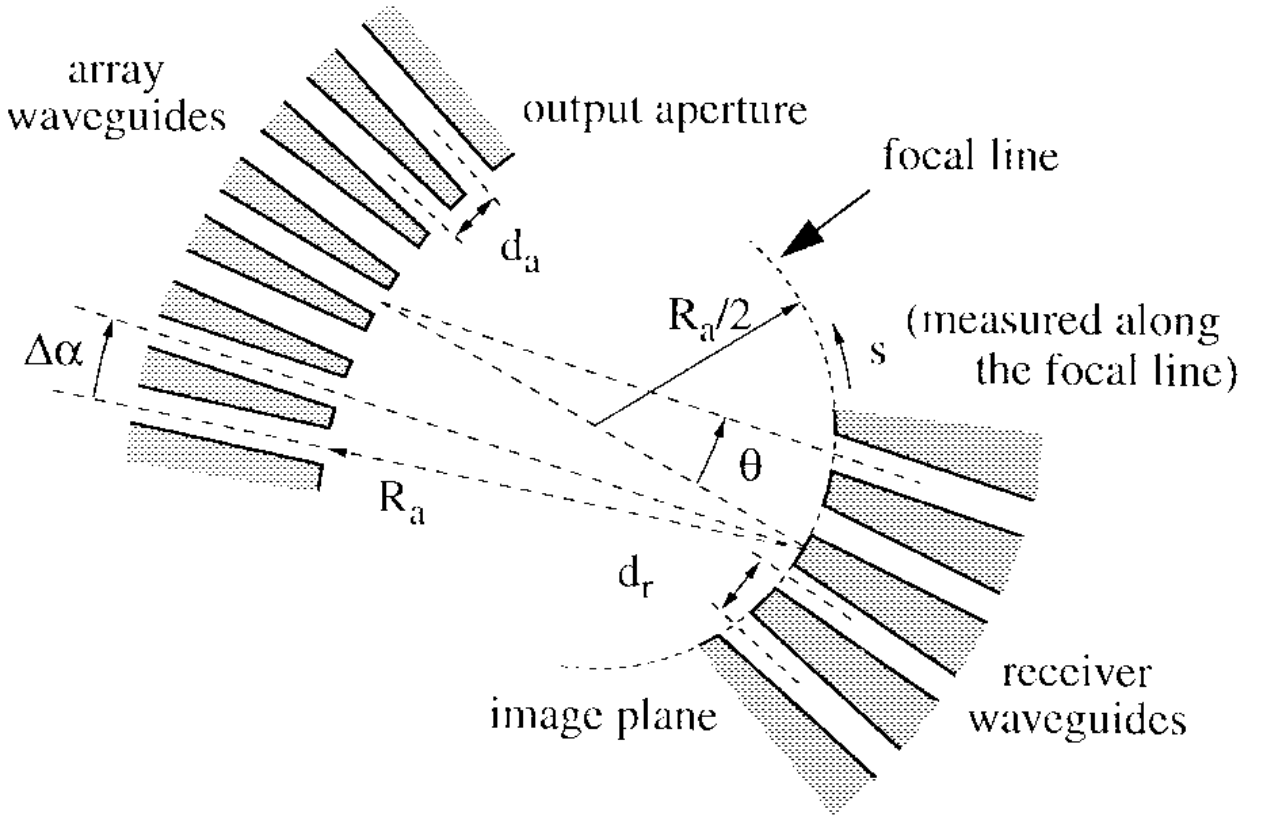
\includegraphics[width=0.4\textwidth]{./object/fprawg.png}
						\caption{Région de propagation libre droite du démultiplexeur}
					}
					
				\end{floatrow}
				\end{figure}

			Ce qu'il faut retenir c'est le fait que les entrées au niveau de la deuxième région de propagation libre agissent similairement à la focale d'une lentille\cite{awg lens}. De plus en raison des différences de longueur des différents guides d'ondes $\ds{\Delta L}$, et leur indice de refraction $\ds{n_g}$ il s'éffectue un décalage de phase $\ds{\Delta \phi}$ entre les differentes ondes. Ce décalage s'exprime de la manière suivante\cite{awg dephase} : \\
			\centerline{$\ds{\Delta \phi= \beta \Delta L}$}
			
			Tel que la constante de propagation des guides d'ondes s'écrit: \\
			\centerline{$\ds{\beta = \frac{2\pi\nu n_{g}}{c}}$}
			
			Par interférence et dispersion des différentes de ses ondes s'établit des franges de diffraction dont la position varie selon la fréquence de l'onde $\ds{f= \frac{c}{\lambda } }$. 
			On peut retrouver cette relation grâce à la dispersion de ce réseau de diffraction comme étant la variation du déplacement sur le plan image par rapport à la variation de fréquence de l'onde \cite{awg dephase}. \\
			\centerline{$\ds{\Delta s = \frac{1}{f_c}\cdot \frac{n_g}{n_{RPL}}\cdot \frac{\Delta L\cdot  R_\alpha }{d_\alpha}\Delta f}$}

			Ainsi pour ce démultiplexage on joue sur la difference de longueur des guides d'ondes pour établir l'espacement entre des différentes chaines permettant de séparer chacune l'une de l'autre afin d'être traitées séparément.

			 

			\subsection{Multiplexage par cristaux photoniques}

			Les cristaux photoniques sont une autre alternative de multiplexage utilisant des tubes diélectriques dans une configuration periodique qui laisse ou bloque les ondes lumineuse de passer. Avec certaines configurations on peut espacer ces tubes de façon à faire des guides d'ondes ou bien extraire certaines longueurs d'ondes en utilisant des cavités de résonance. 

			Ces cavités de résonances sont ajustées de façon à pouvoir absorber une certaine longueur d'onde\cite{PhC} et de la réemetre sur un guide d'onde différent. Sur [Fig.II.4] on peut constater cette architecture avec les cavités de resonances. 

			\begin{figure}[ht!]
				\centering
				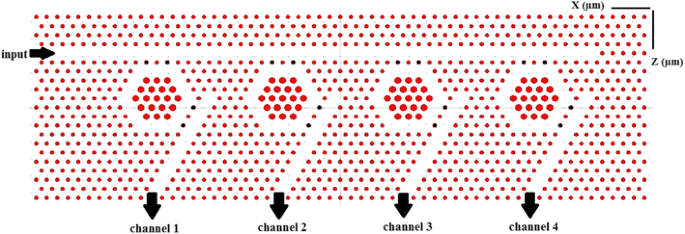
\includegraphics[width=0.7\textwidth]{./object/rescav.png}
				\caption{Architecture d'un cristal photonique}
				\label{fig:rescav}
			\end{figure}
			
			La séparation entre chaque tube diélectrique est donné par $\ds{a_n=a_1- 10^{-9}\cdot(n-1)\text{[nm]} }$ démarquant ainsi pour un démultiplexeur à 8 chaines sur une bande passante de 1550 à 1565 la taille de chaque cavité\cite{PhClen}. 
			\begin{figure}[ht!]
				\centering
				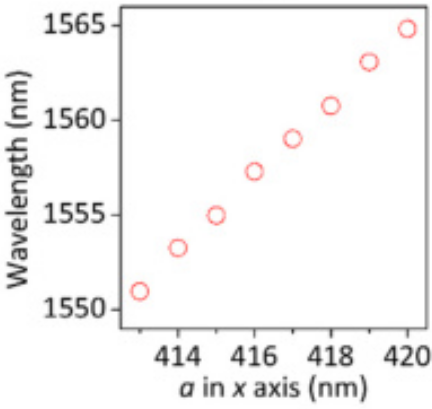
\includegraphics[width=0.2\textwidth]{./object/phclen.png}
				\caption{Taille de la cavité $a$ en fonction de la longueur d'onde sur un cristal photonique}
			\end{figure}

			Cette méthode est réalisable par propriété des cristaux photoniques qui confine les ondes à traverser certain chemin par deconstruction des ondes se propageant et réfléchissant sur les index de réfraction intervalés périodiquement. Cette structure d'index de réfraction périodique établis un retard sur les ondes reflété de manière a`ce que celle ci se déconstruisent dans l'espace, empêchant donc l'onde de se propager autre que sur un chemin prédéterminé. 

			À revoir avec info cours et M2 PhC

		\section{Multiplexage en Polarité}

		\begin{figure}[ht!]
			\centering
			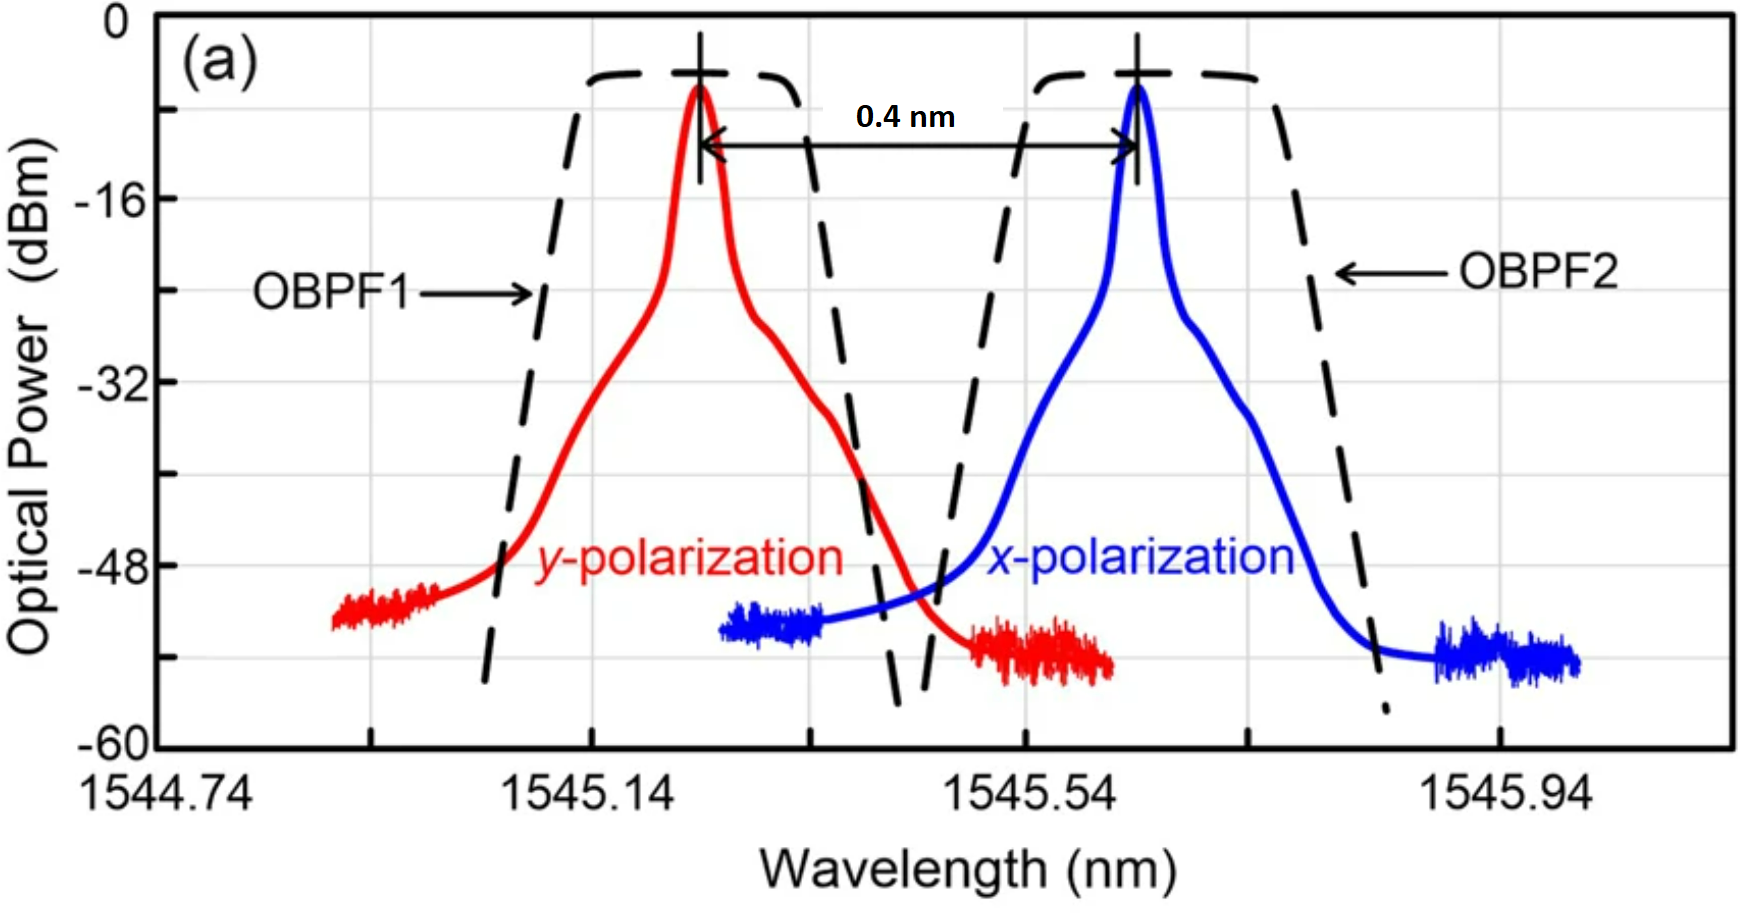
\includegraphics[width=0.5\textwidth]{./object/PDMW.png}
			\caption{Polarisation $x,y$ d'un PDM}
		\end{figure}

		Le PDM est une façon efficace de pouvoir doubler le débit sur une transmission en profitant de la polarisation de la lumière comme un autre intermédiare de multiplexage. Cependant quand on essaie d'appliquer le PDM pour une transmission optique on rencontre un problème d'interférence entre les polarités. Ceci est dû au fait qu'une dipersion du mode de polarisation (PMD) causé par des imperfections dans le milieu de propagation modifie la polarité du signal en fonction de sa fréquence. Plus la ligne de transmission sera longue et plus cette interférence sera importante. On peut exprimer cette modification de la polarité en utilisant les matrices de Jones pour caractériser les polarisations\cite{PDM2}: \\
	\centerline{$\ds{\vec{E}_{out}(\omega)=U_{pol}U_{pmd}\vec{E}_{in}(\omega )}$}

	Avec $\ds{U_{pol}}$ et $\ds{U_{pmd}}$ étant les matrice de Jones caractérisant la polarisation de l'onde et la polarisation engendré par le PMD. 

		C'est pourquoi pour faire marcher le PDM il faut polariser deux longueurs d'ondes differentes, sans séparer ces deux longueurs d'ondes il ne serai pas possible de les démultiplexer en utilisant un filtre à bande passante(OBPF) à cause des interférence entre ces deux polarisations, que l'on appelle le polarisation cross-talk, ce qui peut endommager significativement la performance du multiplexeur\cite{PDM}. 

		La PDM fonctionne cependant grâce au fait que les deux longueurs d'ondes sur lesquelles on effectue la PDM sont espacés d'environ $0.4\ nm$ ce qui est 2 fois plus petit que la séparation $\ds{0.8\ nm}$ entre les longueurs d'onde en WDM dense\cite{DWDM}.Evitant ainsi les interférences entre les longueurs d'onde sur une même polarisation.

		On combine ensuite les deux polarisation pour l'envoyer sur la fibre optique, ensuite lors de la reception du signal on applique simplement un polariseur à bande passante (OBPF) pour que chaque donnée puisse être traités séparámment à la récéption.   

		\section{Multiplexage Temporel}

		\subsection{TDMA}

		\subsection{TDM}

		Étant donné que les composants électroniques ne peuvent supporter des fréquences supérieures à 10 Ghz pour des questions de stabilité, un type de multiplexage a été mis en place : le multiplexage temporel. Ce type de multiplexage permet de combiner plusieurs signaux fonctionnant à des débits peu élevés pour augmenter le débit binaire de transmission. Par la suite, chaque signal se voit affecter l’entièreté de la bande passante durant un court intervalle de temps\cite{wiki1}\cite{wiki2}.

		\begin{figure}[ht!]
			\centering
			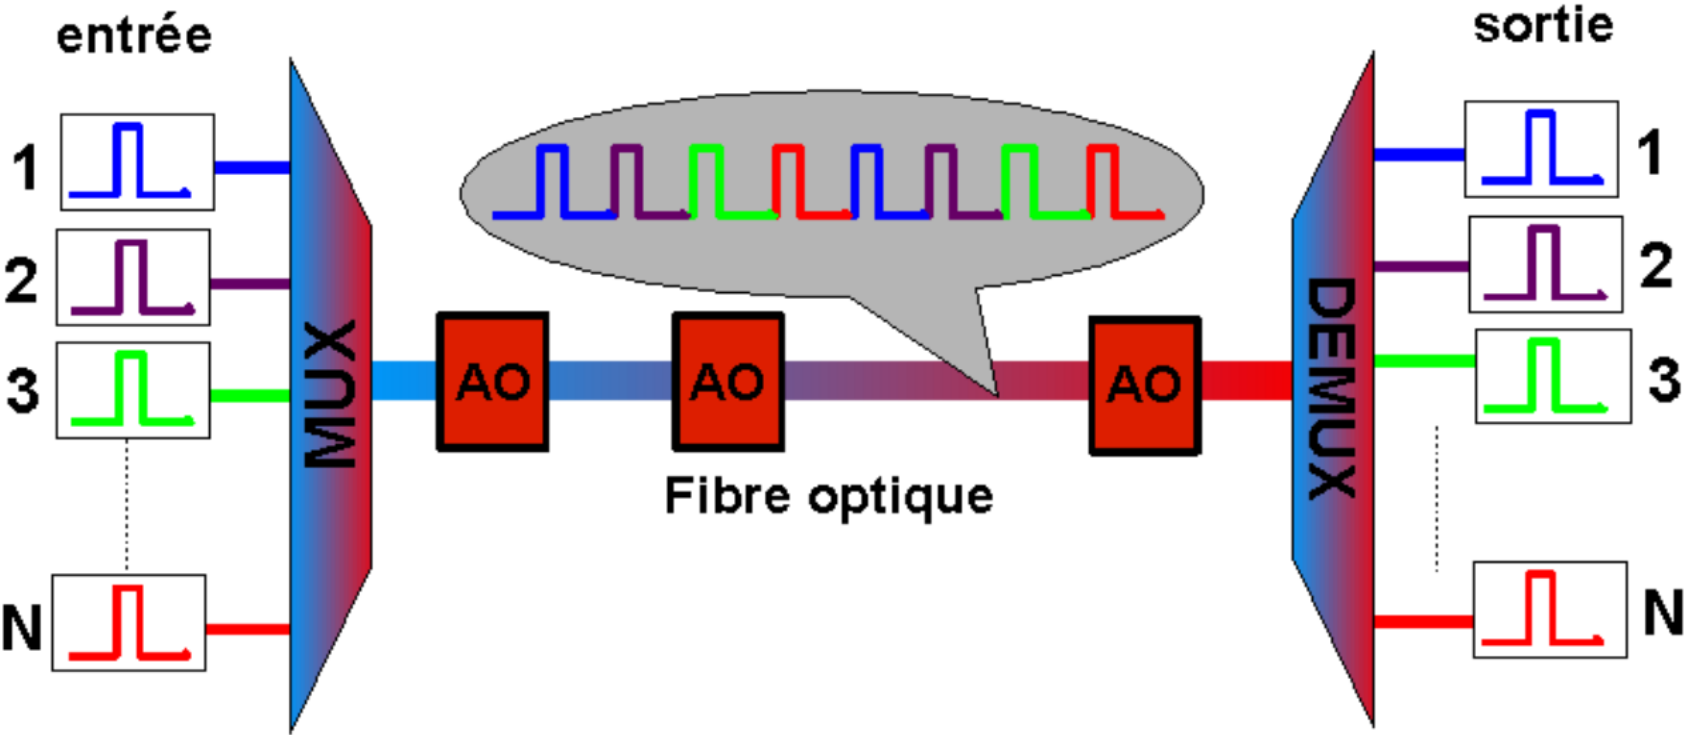
\includegraphics[width=0.5\textwidth]{./object/TDM.png}
			\caption{Schéma TDM}
		\end{figure}

		En revanche, ce qui est réellement utilisé dans le réseau fibre optiques PON, c’est le TDMA (accès multiple par répartition temporelle). C'est-à-dire que chaque client joue le rôle d’un fragment de multiplexeur car il envoie des données de façon à ce qu’elles n’entrent pas en collision avec celles des autres clients.

		\begin{figure}[ht!]
			\centering
			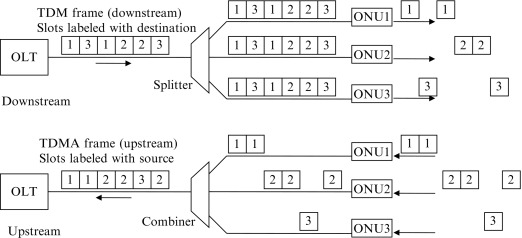
\includegraphics[width=0.5\textwidth]{./object/TDM-A.jpg}
			\caption{DeMux/Mux en TDM et TDMA}
		\end{figure}

		Ce type de multiplexage fonctionne par retard et nécessite que chacun des émetteurs possèdent la même fréquence d’horloge. En revanche, cette fréquence d’horloge doit être déphasée spécifiquement pour chaque client afin de correspondre à un créneau (time-slot) qui lui aura été alloué. L’allocation de créneau se fait généralement dynamiquement, c’est-à-dire que le client reçoit continuellement les nouveaux créneaux qui ne sont plus occupés par les autres clients : cela permet d’optimiser au maximum la bande passante principale.

		\newpage

		\begin{figure}[ht!]
			\centering
			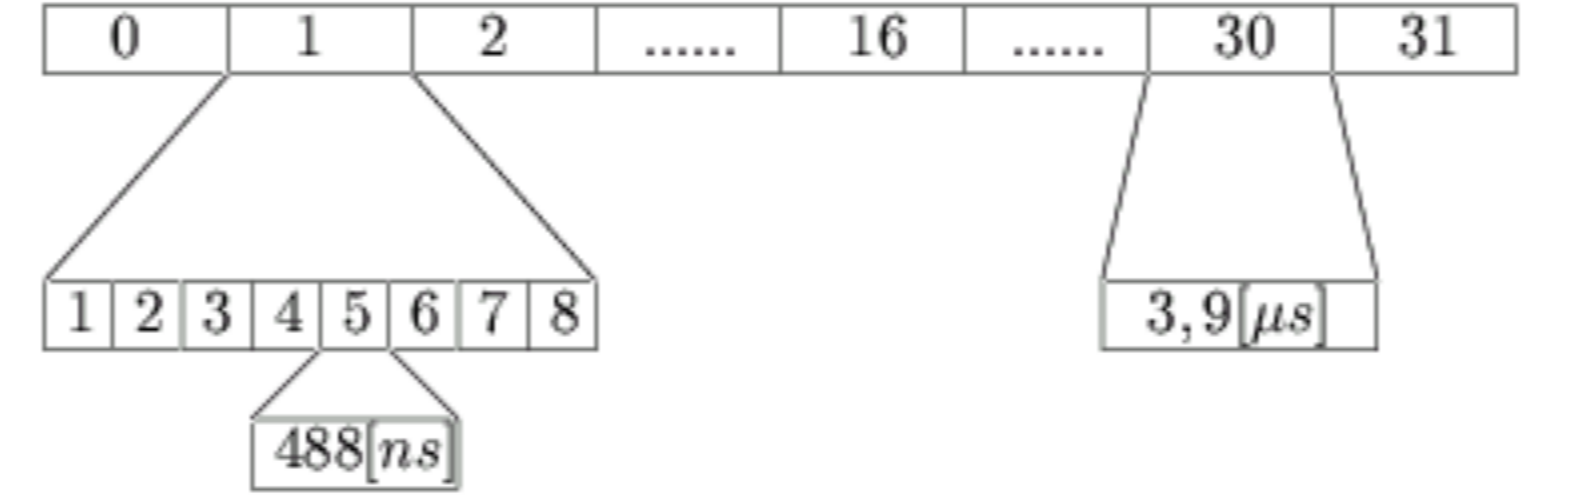
\includegraphics[width=0.4\textwidth]{./object/TDM2.png}
			\caption{Structure de la tramme}
		\end{figure}

		Dans cet exemple, le multiplexage se fait par trame de $3.9\ \mu s$ divisées en 8 créneaux distincts. C’est à dire que chaque créneau a pour durée de $488\ ns$. Ainsi le temps à l’état haut de chaque horloge devra être inférieur de $488\ ns$. Et la fréquence de chaque horloge émettrice sera égale à la fréquence principale divisée par le nombre de créneaux, soit 8 ici. De plus, si l’utilisateur a pour créneau “n” alors il devra appliquer un retard $(n-1)\cdot 488$ à son horloge\cite{cours}.


\chapter{Configuration d'un Réseau PON}

	\vspace{-40pt}
	
		Avant qu’un paquet de données parvienne chez le client d’un fournisseur d’accès internet, celui-ci parcourt de multiples intermédiaires. Nous étudierons une structure de réseau de type PON (passive optical network) FTTH (fiber to the home). C'est-à-dire que plusieurs clients finaux partagent une même fibre optique et que l’utilisateur final possède une fibre optique chez lui en fin de chaîne.
		Plus spécifiquement nous nous pencherons sur la norme GPON (Gigabit PON) créée en 2003 et utilisée par la majorité des opérateurs français pour toutes les offres fibre à destination des particuliers.

		\begin{figure}[ht!]
			\centering
			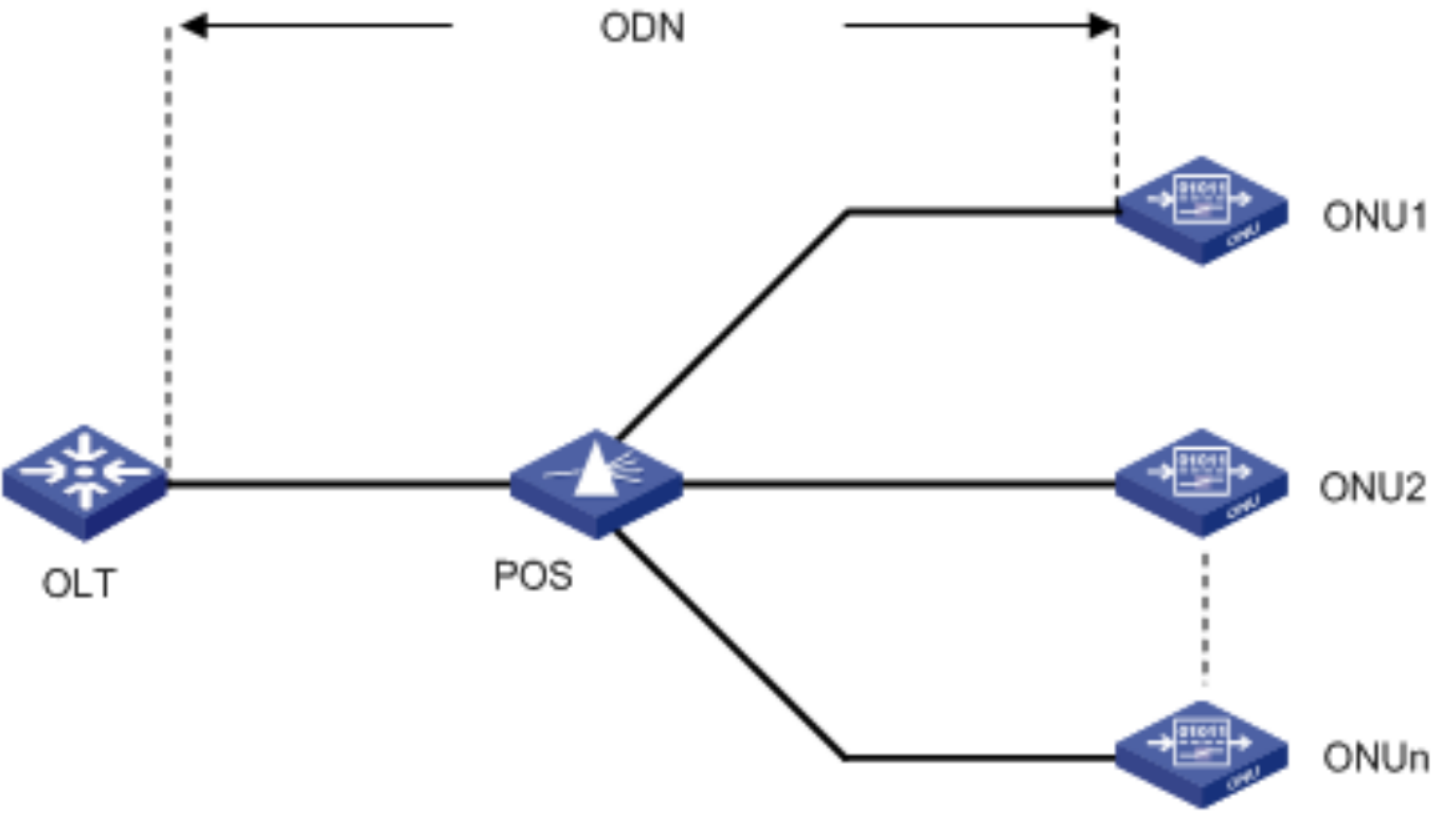
\includegraphics[width=0.45\textwidth]{./object/PON.png}
			\caption{Structure de réseau}
		\end{figure}

		Lorsque un client envoie une information photonique, celle-ci a pour longueur d’onde $1310\ nm$ et lorsqu’il reçoit une information en provenance de l’OLT sa longueur d’onde est de $1490\ nm$. Cela permet un échange d’information bidirectionnel sur une même fibre optique en évitant tout phénomène d’interférence car 2 longueurs d’ondes distinctes sont utilisées.

	\section{Terminal de ligne optique (OLT)}

		Le terminal de ligne optique est le point de départ de tout réseau fibre optique. Celui-ci est chargé de connecter une dorsale internet (backbone) c'est-à-dire un cœur du réseau internet aux clients doté de la technologie fibre optique. Il est surnommé switch optique car sa fonction est la même que le switch ethernet : connecter plusieurs fibre optique à un routeur ancré dans le réseau internet mondial.

		Chaque port permet de connecter une fibre optique qui se partagent entre 32/64/128 clients selon la configuration du PON. Ce partage se fait de façon temporel, c’est à dire que les utilisateurs peuvent utiliser la totalité de la bande passante de la fibre optique principale à tour de rôle : c’est le multiplexage temporel
		Sur l’image ci-dessous le port SFP permet de connecter le switch au réseau mondial.

		\begin{figure}[ht!]
			\centering
			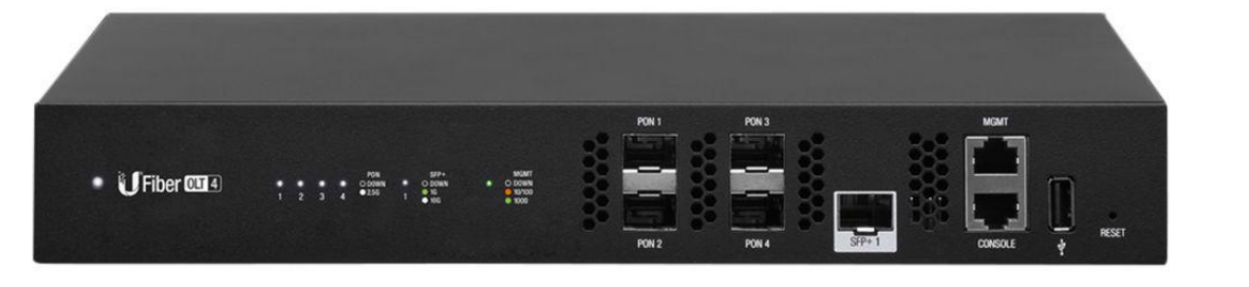
\includegraphics[width=0.5\textwidth]{./object/SFP.png}
			\caption{Image d'un SFP}
		\end{figure}

		Lorsque l’OLT envoie une information à un client, il encapsule l’information de façon chiffrée dans une trame et ajoute en en-tête des informations utiles à la transmission. Cette en-tête contient  entre autres un identifiant permettant d’identifier le receveur.

	\section{Le coupleur (POS)}

		Le coupleur ou Passive Optical Splitter permet d'agréger le signal de plusieurs fibres optiques en une seule ou de cloner le signal d’une fibre optique en plusieurs fibres optiques.
		\begin{figure}[ht!]
			\centering
			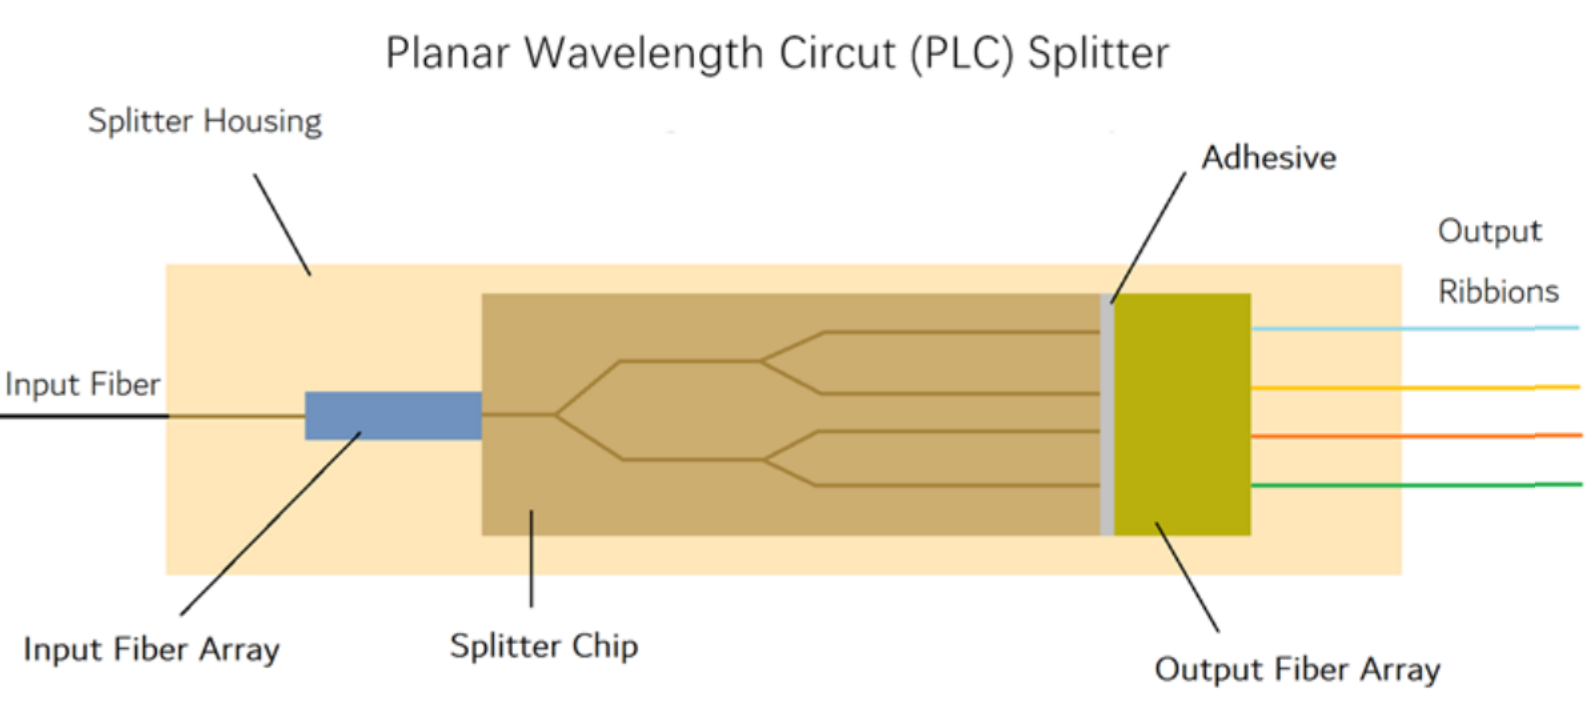
\includegraphics[width=0.6\textwidth]{./object/PLO.png}
			\caption{Passive Optical Splitter}
		\end{figure}

		C’est ce mécanisme qui se produit au niveau des points de mutualisation fibre. En général ces points de mutualisation fibre sont placés dans des armoires électriques dans la rue proche d’habitations ou dans la cave de certains immeubles.

		Lorsque l’OLT envoie les informations de dizaines de clients (ex : téléchargement) sur la même fibre, cette fibre est cloné puis chaque fibre cloné arrive dans l’habitation du client final. Ainsi chaque utilisateur reçoit les informations des dizaines d’autres clients du même point de mutualisation.

		Et lorsque un client envoie des informations à l’OLT (ex : envoie d’un email), la trame va prendre le chemin inverse du précédent, c’est à dire qu’elle va être agrégé à toutes les autres trames des clients pour finir sur la fibre optique de l’OLT.

			
		Ici chaque fibre optique est à destination d’une maison ou d’un appartement et chacun des ports auxquels ces fibres sont branchées transmettent la même information. En effet, chacun des ports transmet la copie du signal envoyé par l’OLT. C’est pour cela qu’un technicien fibre peut se permettre de débrancher votre fibre optique pour brancher celle de votre voisin.



		\section{Le terminal de réseau optique (ONU/ONT)}

		Le terminal de réseau optique est un appareil présent chez chaque client possédant la fibre FTTH.

		\begin{figure}[ht!]
			\centering
			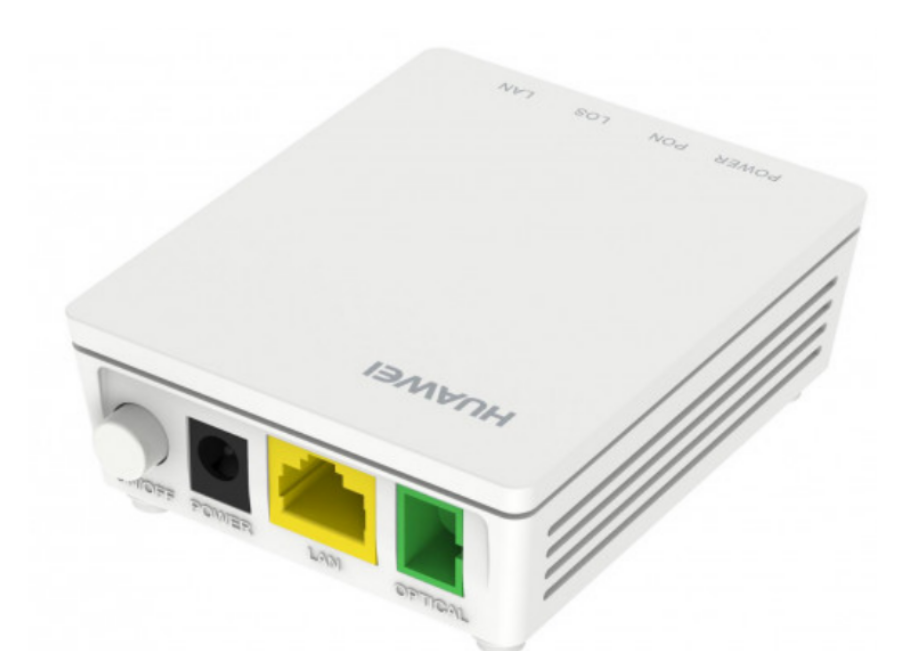
\includegraphics[width=0.2\textwidth]{./object/cables.png}
			\caption{Terminal de réseau optique}
		\end{figure}
		
		\vspace{3cm}

		Celui-ci comprend un port fibre dont une fibre reliée au splitter précédemment évoqué, ainsi qu’un port Ethernet relié à la box internet.

		Lorsque le client reçoit une information :
		\begin{items}{-15pt}{-15pt}
			\item Le signal photonique est démultiplexé temporellement
			\item Le signal démultiplexé est modulé en signal électrique
			\item Si l’en-tête de la trame GPON correspond à l’identifiant de l’ONT alors l’information encapsulée sera déchiffrée via une clé préalablement échangée avec l’OLT.
			\item  Puis l’information sera mise sous forme d’une trame interprétable par le routeur, et envoyé via le port Ethernet
		\end{items}
		
		Lorsque le client envoie une information :
		\begin{items}{-15pt}{-15pt}
		\item La trame Ethernet est encapsulée de façon à la chiffrer et à ajouter une en-tête contenant l’identifiant de l’ONT.
		\item Cette trame est modulé en signal photonique et multiplexé temporellement
		\item  Ensuite elle est envoyée via le port optique au point de mutualisation en vue d'être agrégé sur la fibre central de l’OLT.
			
		\end{items}

		\section{Bilan et Conclusion}




			\clearpage
			\pagestyle{bib}
			\begin{thebibliography}{9}

				\bibitem{attenuation}
				Khushbu Solanki, Livre Blanc, Fibre Optics vs Copper Cabling – Understanding the Difference, OptronicsPlus

				\bibitem{Open}
				Dasan, M. et al., 2019, 'Optically Multiplexed Systems: Wavelength Division Multiplexing', in S. Mohammady (ed.), Multiplexing, IntechOpen, London. 10.5772/intechopen.88086.

				\bibitem{awg lens}
				Leijtens, X. J. M., Kuhlow, B., \& Smit, M. K. (2006). Arrayed waveguide gratings. In H. Venghaus (Ed.), Wavelength filters in fiber optics (pp. 125-187).

				\bibitem{awg dephase}
				Smit, M. K., \& Dam, van, C. (1996). PHASAR-based WDM-devices: principles, design and applications. IEEE. Journal of Selected Topics in Quantum Electronics, 2(2), 236-250.

				\bibitem{PhC}
				Jessie Rosenberg, Rajeev V. Shenoi, Sanjay Krishna, and Oskar Painter, "Design of plasmonic photonic crystal resonant cavities for polarization sensitive infrared photodetectors," Opt. Express 18, 3672-3686 (2010)


				\bibitem{PhClen}
				Yuta Ooka, Tomohiro Tetsumoto, Nurul Ashikin Binti Daud, and Takasumi Tanabe, "Ultrasmall in-plane photonic crystal demultiplexers fabricated with photolithography," Opt. Express 25, 1521-1528 (2017)

				\bibitem{PDM2}
				Zinan Wang, Chongjin Xie, and Xiaomin Ren, "PMD and PDL impairments in polarization division multiplexing signals with direct detection," Opt. Express 17, 7993-8004 (2009)

				\bibitem{PDM}
				Wu, HW., Li, CY., Lu, HH. et al. A PDM-based 128-Gb/s PAM4 fibre-FSO convergent system with OBPFs for polarisation de-multiplexing. Sci Rep 10, 1872 (2020). https://doi.org/10.1038/s41598-020-58558-7

				\bibitem{DWDM}
				Article, SmartOptics, "COARSE AND DENSE WAVELENGTH DIVISION MULTIPLEXING", accédé le 08/12/2022

				\bibitem{telecom}
				 Optical Fiber Telecommunications Volume VIB par Kaminow, Ivan P. en 2013
(ISBN : 978-0-12-396960-6)

				\bibitem{prot}
				Réseaux et transmissions, Protocoles, infrastructures et services, Lohier Stéphane,
Présent Dominique en 2020 (ISBN : 978-2-10-081183-0)

				\bibitem{cours}
				Cours sur le multiplexage temporel http://www.telecom.ulg.ac.be/teaching/notes/total0/elen036/node170\_mn.html

				\bibitem{wiki1}
				https://en.wikipedia.org/wiki/Time-division\_multiple\_access

				\bibitem{wiki2}
				https://fr.wikipedia.org/wiki/Acc\%C3\%A8s\_multiple\_par\_r\%C3\%A9partition\_temporelle
		\end{thebibliography}




	
\end{document}
